\documentclass[aspectratio=169,11pt]{beamer}
\usetheme{Madrid}
\usecolortheme{default}
\usepackage{amsmath,graphicx,booktabs}

\graphicspath{{figures/}}

\definecolor{IEEEblue}{RGB}{0,75,135}
\setbeamercolor{structure}{fg=IEEEblue}
\setbeamercolor{frametitle}{fg=white,bg=IEEEblue}
\setbeamercolor{title}{fg=white,bg=IEEEblue}
\setbeamercolor{subtitle}{fg=white,bg=IEEEblue}
\setbeamertemplate{navigation symbols}{}
\setbeamertemplate{footline}[frame number]

\title[GapSSM: Missing-Frame EF Prediction]{GapSSM: Missing-Frame-Aware Ejection Fraction Prediction from Echocardiography Videos}
\subtitle{Baseline (R3D-18) vs.\ Proposed Mamba (\textsc{GapSSM}) on EchoNet-Dynamic}
\author{Deepak Kumar \quad $\bullet$ \quad Kalki Dang \quad $\bullet$ \quad Aryan Solanki}
\institute{Department of Computer Science and Engineering\\Project 6: Cardiac Function Prediction with Missing Frames}
\date{November 2026}

\begin{document}

\begin{frame}[plain]
\titlepage
\end{frame}

\begin{frame}{Presentation Roadmap}
\tableofcontents
\end{frame}

\section{Problem and Motivation}
\begin{frame}{Problem Statement \& Clinical Motivation}
\begin{itemize}
    \item \textbf{Goal:} Directly regress Left-Ventricular Ejection Fraction ($\text{EF} = (\text{EDV}-\text{ESV})/\text{EDV}\times 100$) from a $32$-frame grayscale echocardiography clip.
    \item \textbf{Clinical Challenge:} Ultrasound recordings frequently drop frames due to low frame rates, probe movement, compression artifacts, or acoustic shadowing.
    \item \textbf{Why Missing Frames Matter:} EF depends on End-Diastole (ED) and End-Systole (ES); missing frames around ES/ED distort EF estimates.
    \item \textbf{Gap in Prior Work:} Standard 3D CNNs (R3D-18) assume uniform temporal grids and degrade sharply when frames are missing.
\end{itemize}
\end{frame}

\section{Objectives and Prior Work}
\begin{frame}{Objectives \& Related Work}
\begin{columns}
\column{0.52\textwidth}
\textbf{Project Objectives}
\begin{itemize}
    \item Build a reproducible R3D-18 complete-video baseline on EchoNet-Dynamic.
    \item Propose \textsc{GapSSM}, a missing-frame-aware selective state-space model.
    \item Compare both across MAE, MSE, RMSE, $R^2$, MAPE, Pearson $r$, bias, shift, AUC, MC uncertainty, and efficiency.
\end{itemize}
\column{0.45\textwidth}
\begin{table}\centering\scriptsize
\caption{Reference Literature Context}
\begin{tabular}{p{2.3cm}p{2.7cm}}\toprule
Reference & Role in Project \\\midrule
EchoNet-Dynamic (2019/2020) & $10,030$ videos; R(2+1)D / R3D MAE $4.22$, $R^2=0.79$ \\
Mamba (2023) & Selective SSMs with continuous-time $\Delta_t$ \\
VideoMamba (2024) & SSMs for video; \textsc{GapSSM} adds gap decay + state hold \\
EchoForge / OSA (CVPR 2025) & Ultrasound speckle & temporal drift motivation \\
\bottomrule
\end{tabular}
\end{table}
\end{columns}
\end{frame}

\section{Approach}
\begin{frame}{Proposed Method: \textsc{GapSSM} Architecture}
\begin{itemize}
    \item \textbf{1. Mask-Gated Frame Encoder:} GroupNorm ResNet-18 encodes \emph{only} observed frames ($m_t=1$); unobserved frames never enter the spatial encoder or causal 1D conv.
    \item \textbf{2. Continuous-Time Gap Decay:} Across multi-step gaps $\Delta\tau_t = \tau_t - \tau_{\text{last}}$, state $\mathbf{h}_{t-1}$ decays via learned per-channel rates $\mathbf{r}_{\text{gap}}$:
    \[
        \mathbf{h}_{\text{before}} = \exp\bigl(\mathbf{A} \odot \text{softplus}(\mathbf{r}_{\text{gap}}) \cdot \max(0, \Delta\tau_t - 1)\bigr) \odot \mathbf{h}_{t-1}
    \]
    \item \textbf{3. State Holding (\texttt{hold\_missing}):} When $m_t=0$, $\mathbf{h}_t = \mathbf{h}_{t-1}$ and $\tau_{\text{last}}$ is preserved.
    \item \textbf{4. ZOH Selective Update & Pooling:} Exact zero-order-hold update + masked mean pooling over observed frames.
\end{itemize}
\end{frame}

\begin{frame}{Experimental Setup & Training Workflow}
\begin{columns}
\column{0.52\textwidth}
\begin{itemize}
    \item \textbf{Dataset:} EchoNet-Dynamic ($10,030$ videos, $112\times 112$, $32$ frames at stride $2$).
    \item \textbf{Official Split:} $7,465$ Train / $1,288$ Val / Paired Test ($N=200$ \texttt{main}, $N=98$ \texttt{phase}).
    \item \textbf{Test Conditions:} Ratios $\{0\%, 10\%, 25\%, 50\%, 75\%\}$; patterns (\texttt{random}, \texttt{block}, \texttt{ed}, \texttt{es}, \texttt{systole}, \texttt{diastole}); $4$ handlings (\texttt{zero}, \texttt{removal}, \texttt{repeat}, \texttt{interpolate}); MC Dropout.
\end{itemize}
\column{0.45\textwidth}
\begin{table}\centering\scriptsize
\caption{Model & Training Summary}
\begin{tabular}{lcc}\toprule
Property & Baseline (R3D-18) & \textsc{GapSSM} \\\midrule
Parameters & 33.17M & \textbf{11.39M} \\
Train Corruption & No & Yes \\
Epochs Run & 24 & 15 \\
Best Val MAE & \textbf{5.08 pp} & 6.69 pp \\
Peak Train GPU & 2.13 GB & \textbf{2.03 GB} \\
Inf.\ Time / Cond. & 12.47 ms & \textbf{8.43 ms} \\
\bottomrule
\end{tabular}
\end{table}
\end{columns}
\end{frame}

\section{Experiments and Results}
\begin{frame}{Training Curves: Loss \& Validation MAE}
\begin{center}
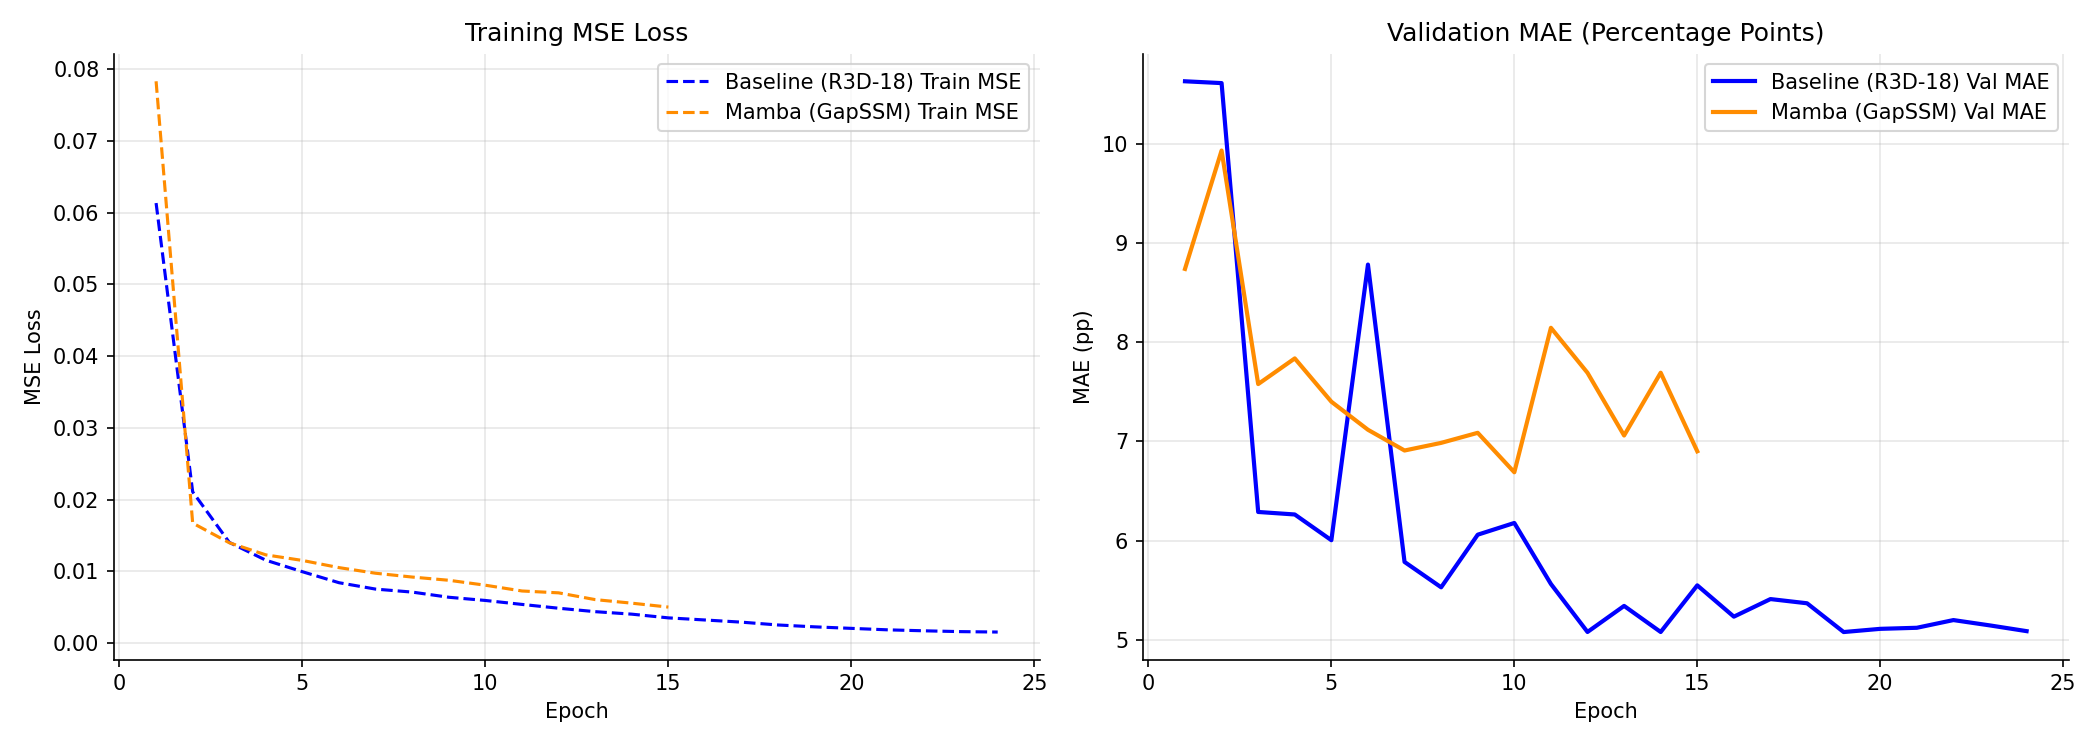
\includegraphics[width=0.92\textwidth,height=0.72\textheight,keepaspectratio]{training_comparison.png}
\end{center}
\end{frame}

\begin{frame}{Random Missing Frames: All 8 Metrics (\texttt{zero}, $N=200$)}
\begin{center}
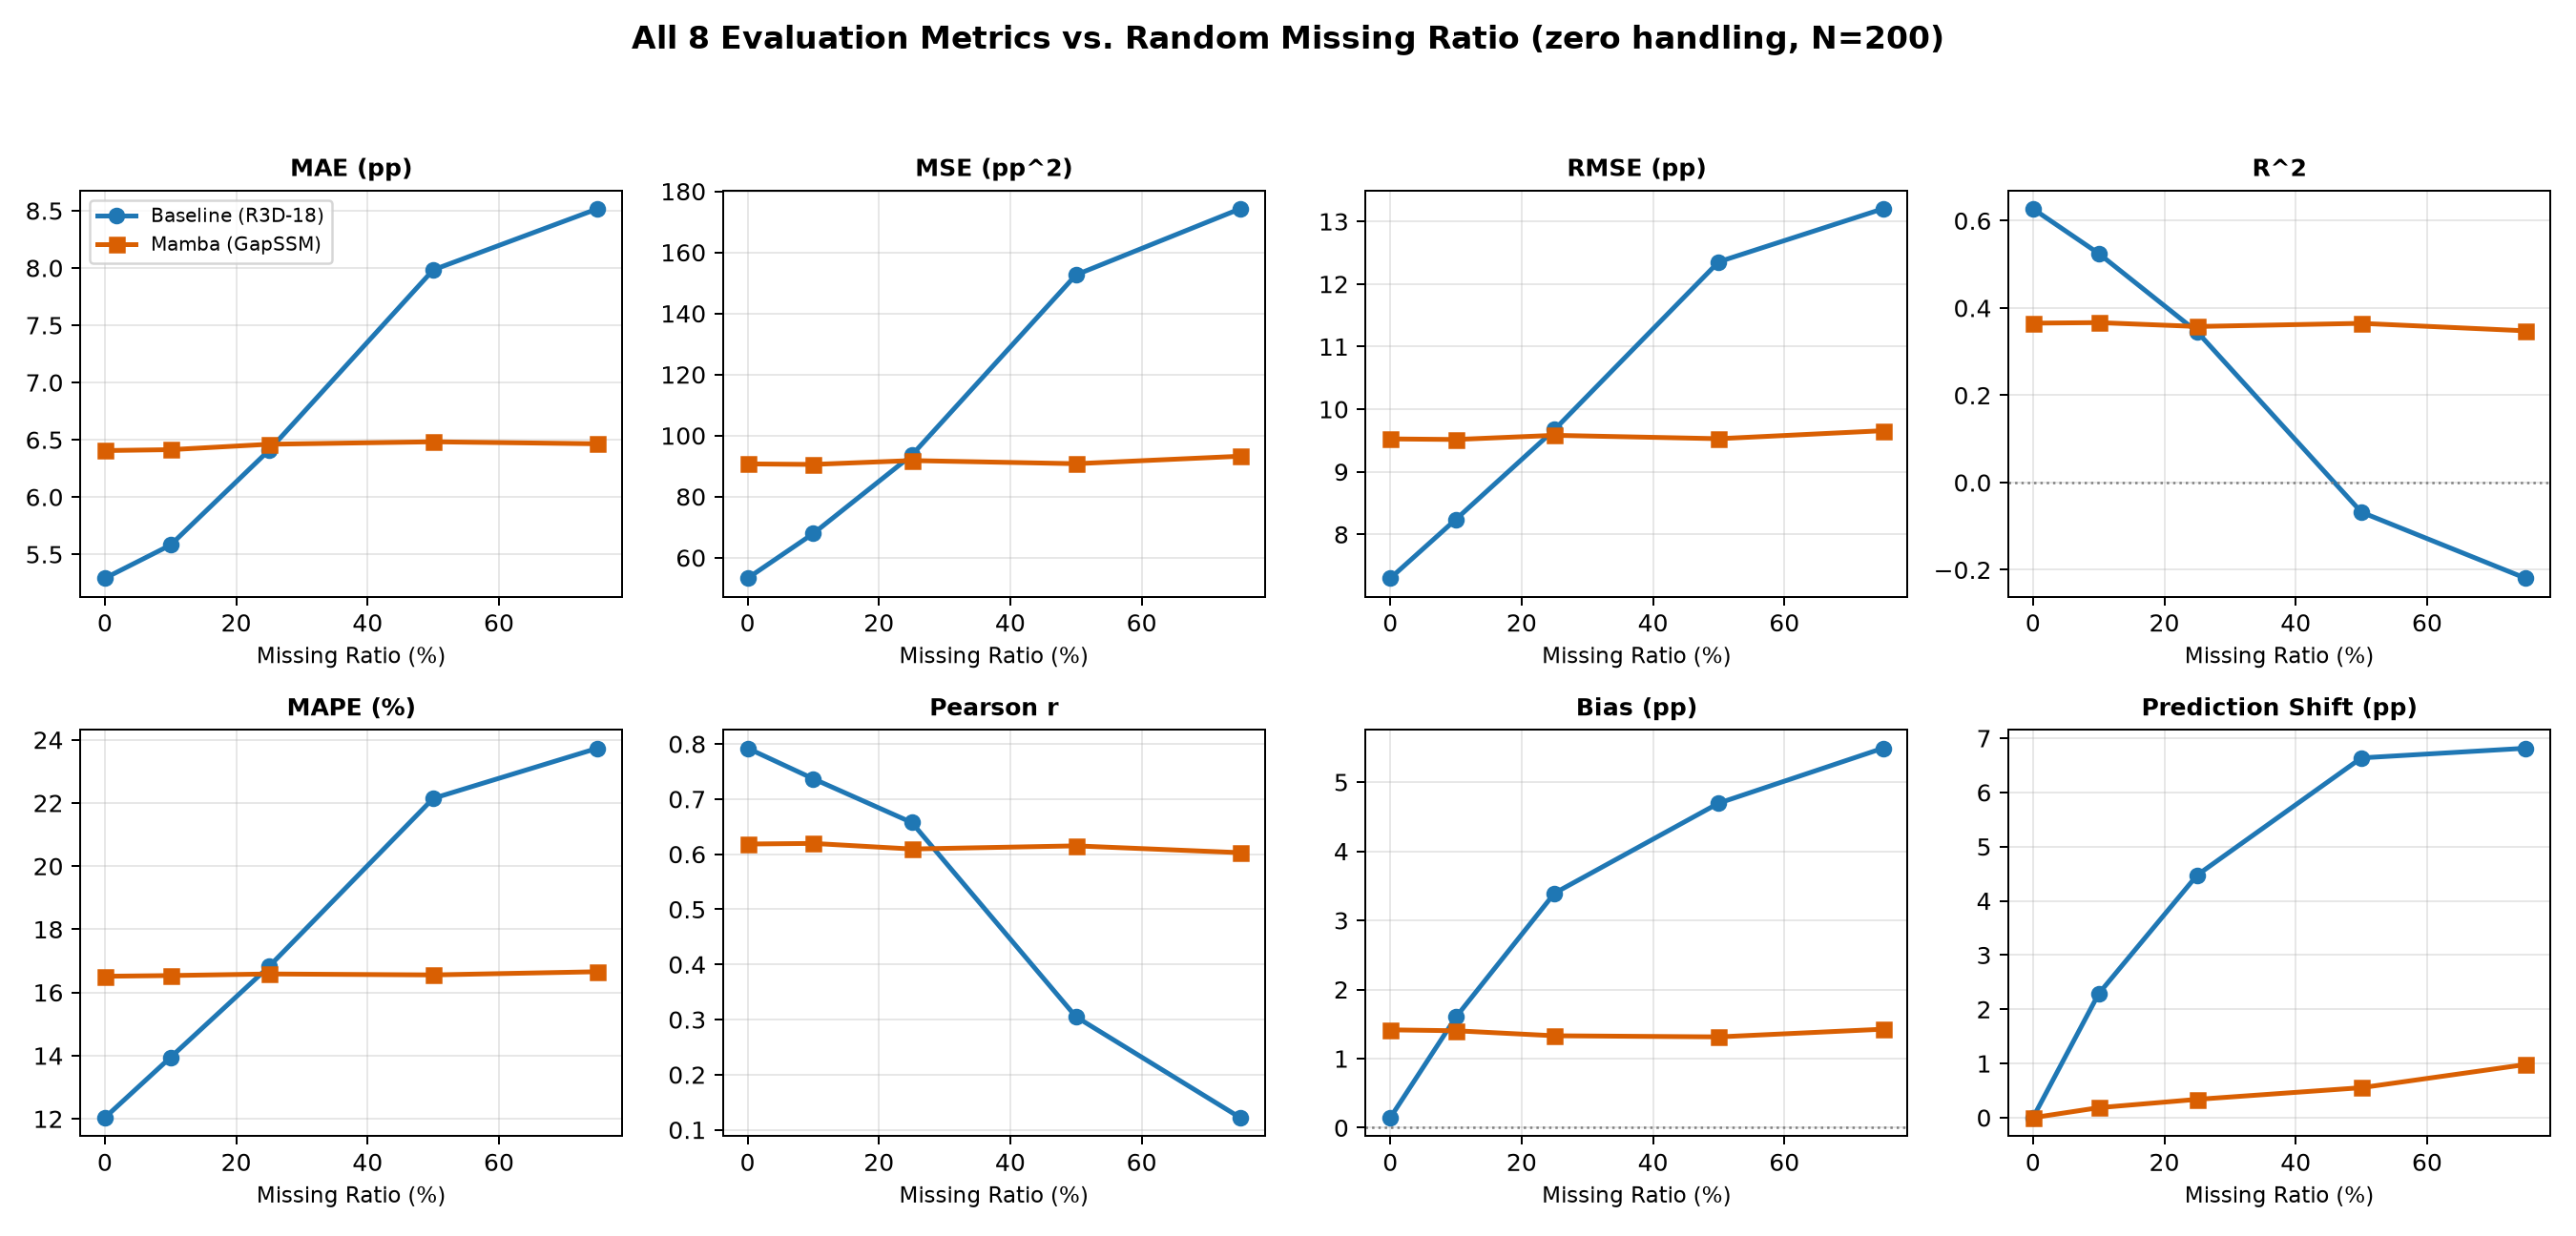
\includegraphics[width=0.95\textwidth,height=0.72\textheight,keepaspectratio]{fig_metrics_random.png}
\end{center}
\end{frame}

\begin{frame}{Consecutive Block Missing Frames: All 8 Metrics (\texttt{zero}, $N=200$)}
\begin{center}
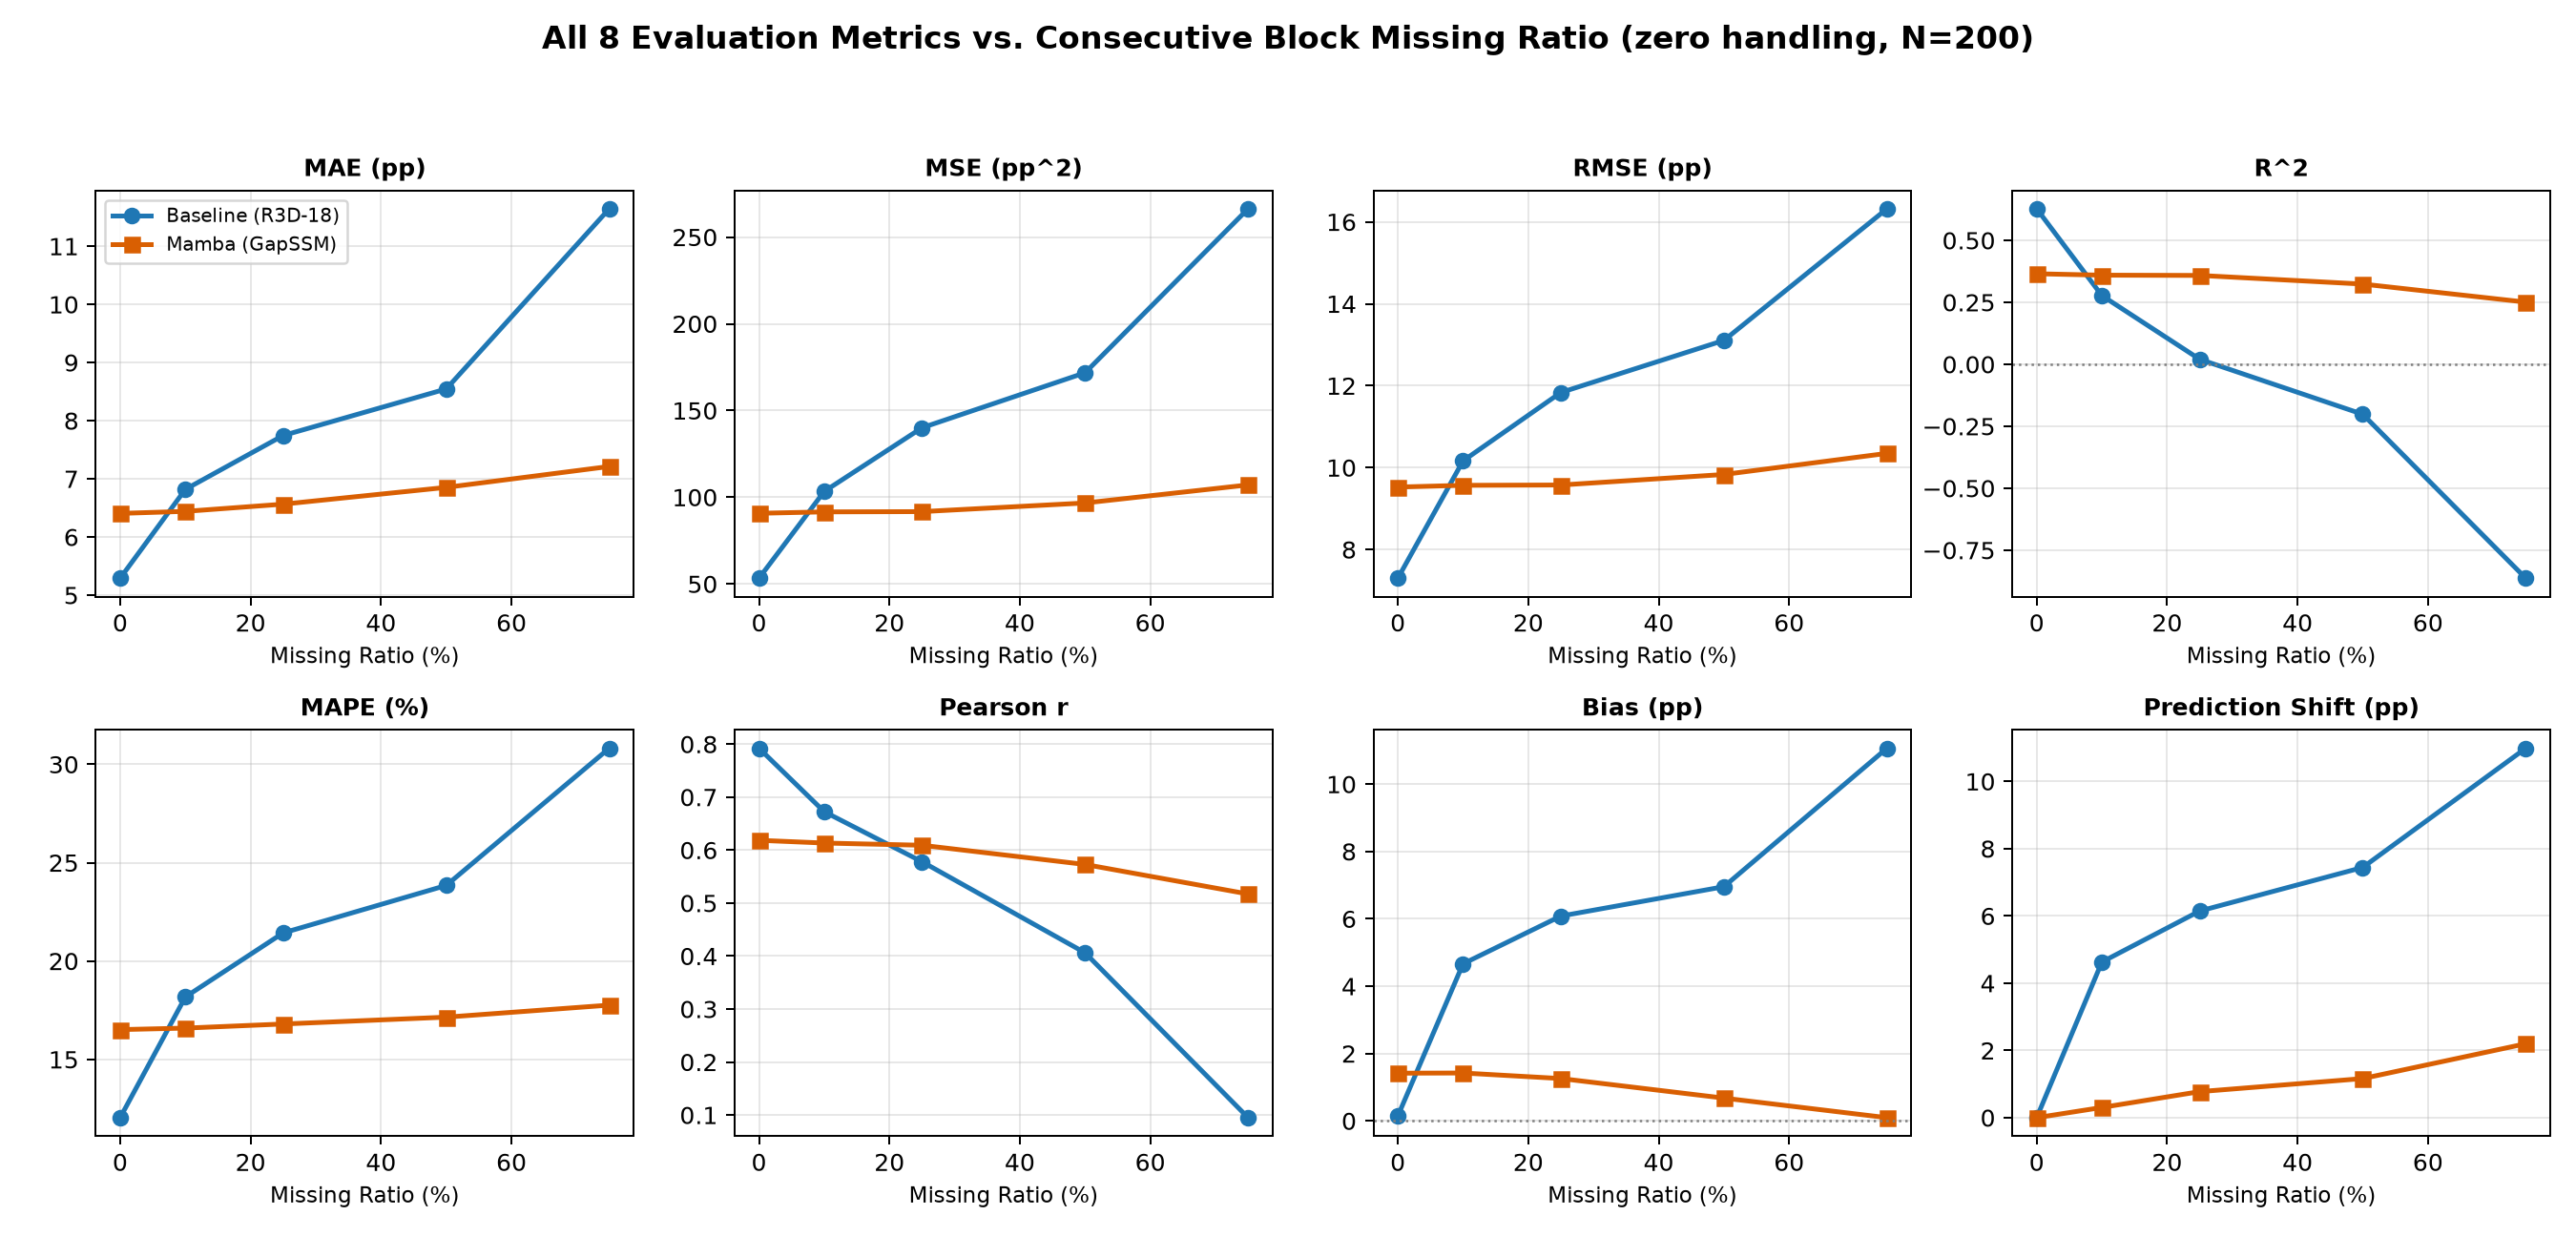
\includegraphics[width=0.95\textwidth,height=0.72\textheight,keepaspectratio]{fig_metrics_block.png}
\end{center}
\end{frame}

\begin{frame}{Complete vs.\ Missing-Frame Quantitative Comparison ($N=200$)}
\begin{table}\centering\scriptsize
\begin{tabular}{llcccccc}\toprule
Model & Pattern & Ratio & MAE $\downarrow$ & RMSE $\downarrow$ & $R^2 \uparrow$ & $\Delta$MAE & Pred Shift \\\midrule
Baseline & \texttt{random} & 0.00 & \textbf{5.29} & \textbf{7.30} & \textbf{0.627} & 0.00 & 0.00 \\
Baseline & \texttt{random} & 0.75 & 8.52 & 13.20 & -0.219 & +3.23 & 6.82 \\
\textsc{GapSSM} & \texttt{random} & 0.00 & 6.41 & 9.53 & 0.365 & 0.00 & 0.00 \\
\textsc{GapSSM} & \texttt{random} & 0.75 & \textbf{6.46} & \textbf{9.66} & \textbf{0.348} & \textbf{+0.06} & \textbf{0.98} \\\midrule
Baseline & \texttt{block} & 0.25 & 7.75 & 11.83 & 0.020 & +2.45 & 6.15 \\
Baseline & \texttt{block} & 0.75 & 11.64 & 16.32 & -0.863 & +6.35 & 10.99 \\
\textsc{GapSSM} & \texttt{block} & 0.25 & \textbf{6.56} & \textbf{9.58} & \textbf{0.358} & \textbf{+0.16} & \textbf{0.77} \\
\textsc{GapSSM} & \texttt{block} & 0.75 & \textbf{7.21} & \textbf{10.35} & \textbf{0.251} & \textbf{+0.81} & \textbf{2.20} \\
\bottomrule
\end{tabular}
\end{table}
\vspace{0.3em}
\begin{itemize}\small
    \item \textbf{Honest Finding:} R3D-18 leads on complete clips ($5.29$ vs.\ $6.41$~pp), while \textsc{GapSSM} cuts $75\%$-block degradation by $87.2\%$ and prediction shift by $80.0\%$.
\end{itemize}
\end{frame}

\begin{frame}{Additional Evaluations: Degradation, AUC Robustness & Uncertainty}
\begin{center}
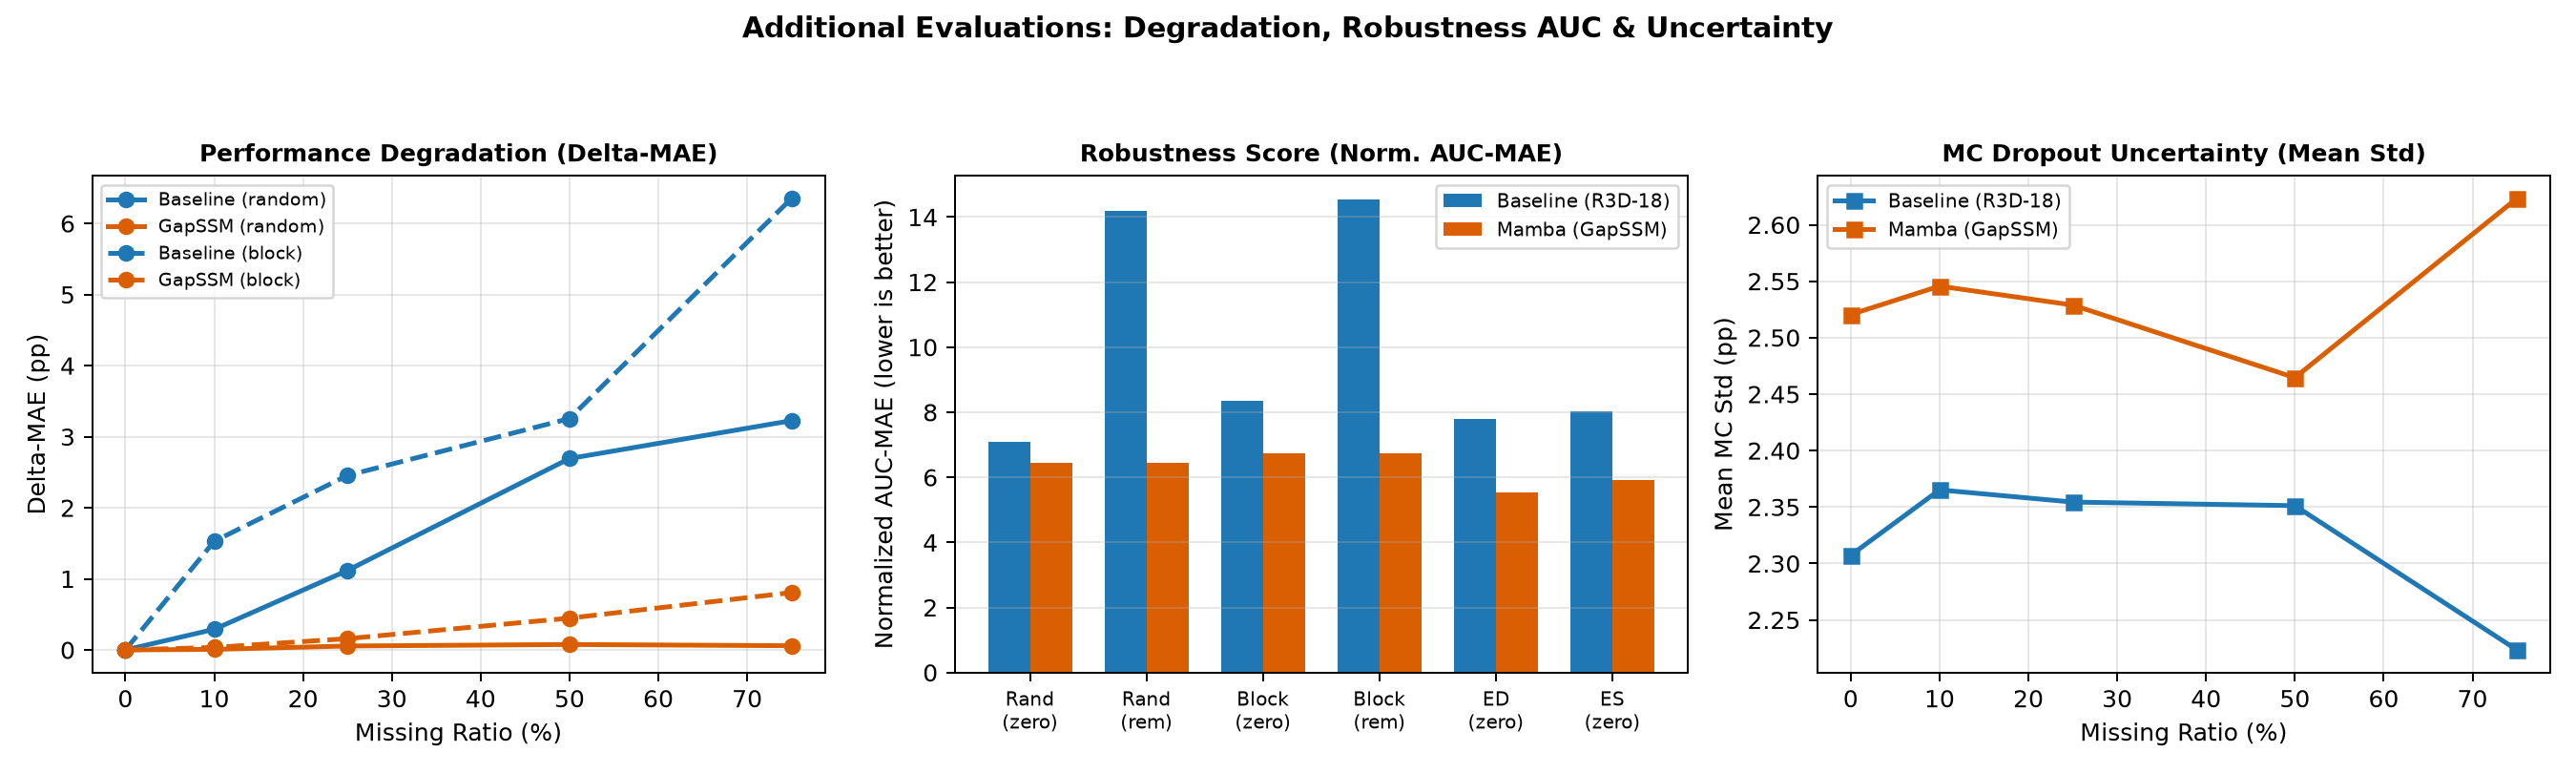
\includegraphics[width=0.95\textwidth,height=0.68\textheight,keepaspectratio]{fig_robustness_degradation.png}
\end{center}
\end{frame}

\begin{frame}{Cardiac-Phase Sensitivity, Input Handling & Clinical UI}
\begin{columns}
\column{0.50\textwidth}
\begin{table}\centering\scriptsize
\caption{25\% Phase Missingness (\texttt{zero}, $N=98$)}
\begin{tabular}{lccc}\toprule
Position & Baseline MAE & \textsc{GapSSM} MAE & Shift (B/M) \\\midrule
Complete & \textbf{3.78} & 5.60 & 0.00 / 0.00 \\
\texttt{ed} & 8.27 & \textbf{5.49} & 7.19 / \textbf{0.95} \\
\texttt{es} & 7.17 & \textbf{5.96} & 5.62 / \textbf{0.86} \\
\texttt{systole} & 8.02 & \textbf{5.63} & 7.02 / \textbf{0.67} \\
\texttt{diastole} & 7.26 & \textbf{5.81} & 6.32 / \textbf{0.64} \\
\bottomrule
\end{tabular}
\end{table}
\column{0.48\textwidth}
\begin{itemize}\small
    \item \textbf{Handling Invariance:} \textsc{GapSSM} achieves identical MAE ($6.56$~pp) across \texttt{zero}, \texttt{repeat}, \texttt{interpolate}, and \texttt{removal} at $25\%$ block loss.
    \item \textbf{Clinical UI (\texttt{app.py}):} Interactive Gradio web app for \texttt{.avi}/\texttt{.mp4} upload, EF + MC uncertainty output, and missing-frame simulation.
\end{itemize}
\end{columns}
\end{frame}

\section{Conclusion}
\begin{frame}{Limitations, Conclusion \& Future Work}
\begin{itemize}
    \item \textbf{Conclusion:} \textsc{GapSSM} is dramatically more robust than R3D-18 under random, block, and phase-specific missing frames ($\Delta\text{MAE}=+0.06$~pp at $75\%$ random; $+0.81$~pp at $75\%$ block) with $2.9\times$ fewer parameters ($11.39$M vs.\ $33.17$M) and faster inference ($8.43$ vs.\ $12.47$~ms).
    \item \textbf{Limitations:} Paired $200$-video test subset; single seed; un-pretrained GroupNorm ResNet-18 encoder; unidirectional SSM.
    \item \textbf{Future Work:} ImageNet-pretrained 2D encoder, bidirectional SSM + mean/max pooling to close the $0\%$ gap, and full $1,288$-video test evaluation.
\end{itemize}
\end{frame}

\begin{frame}{References \& Questions}
\scriptsize
\begin{itemize}
    \item[{[1]}] D. Ouyang et al., ``Video-based AI for beat-to-beat assessment of cardiac function,'' \textit{Nature}, vol. 580, pp. 252--256, 2020.
    \item[{[2]}] D. Ouyang et al., ``EchoNet-Dynamic: a large new cardiac motion video data resource,'' \textit{NeurIPS ML4H}, 2019.
    \item[{[3]}] A. Gu and T. Dao, ``Mamba: Linear-time sequence modeling with selective state spaces,'' \textit{arXiv:2312.00752}, 2023.
    \item[{[4]}] K. Li et al., ``VideoMamba: State space model for efficient video understanding,'' \textit{ECCV}, 2024.
    \item[{[5]}] Y. Gal and Z. Ghahramani, ``Dropout as a Bayesian approximation,'' \textit{ICML}, 2016.
    \item[{[6]}] Y. Fang et al., ``EchoForge,'' \textit{CVPR}, 2025; R. Wang et al., ``OSA,'' \textit{CVPR}, 2025.
\end{itemize}
\vspace{0.8em}
\centering\normalsize\textbf{Thank You --- Questions?}\\
\small Deepak Kumar $\bullet$ Kalki Dang $\bullet$ Aryan Solanki
\end{frame}

\end{document}
